
Adding a user, is a feature only available for the admin user and is a crucial use-case needed for saving a new user’s to the system.
\newline
\newline
The add user case passed unit testing successfully as seen in the figure bellow
\newline
\newline
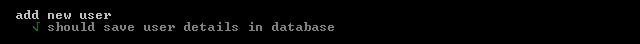
\includegraphics[width=350px]{./Graphics/addUser}
\newline		
\subsubsection*{Conditions}
The following pre and post conditions are defined for adding a new user.
\newline
\newline	
\subsubsection*{Pre conditions}	
\begin{itemize}
		\item User must be logged in as admin.
		\item User to be added must not already exist in the database.
		\item User must be a medical personnel.
\end{itemize}	

\subsubsection*{Post conditions}	
\begin{itemize}
		\item New user is added and can interact with the system.
\end{itemize}	

The code bellow shows the testing for adding a new user with sample data	
\newline
\newline
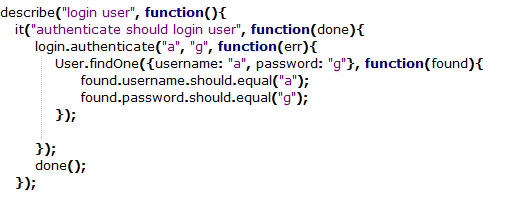
\includegraphics[width=350px]{./Graphics/UserMustLogIn}

\subsubsection*{Remark}
Add User unit test successfully passes.